\chapter{Abrasione}\label{chp:Abrasione}
Nell'abrasione, a differenza dell'asportazione di truciolo, i taglienti sono piccoli e dispersi casualmente nell'utensile.
In più i trucioli sono piccoli, come delle polveri.
Si ha per forza una profondità di passata molto piccola, per cui l'energia specifica della lavorazione è molto alta.
Dunque sono molto inefficienti per via del fatto che devo spendere tanta energia per rimuovere il materiale.
Siccome l'energia dipende dallo spessore di truciolo indeformato, il fatto che venga asportato pochissimo spessore motiva l'alata energia specifica.
Per fortuna se ne deve rimuovere molto poco.

\begin{figure}
\centering
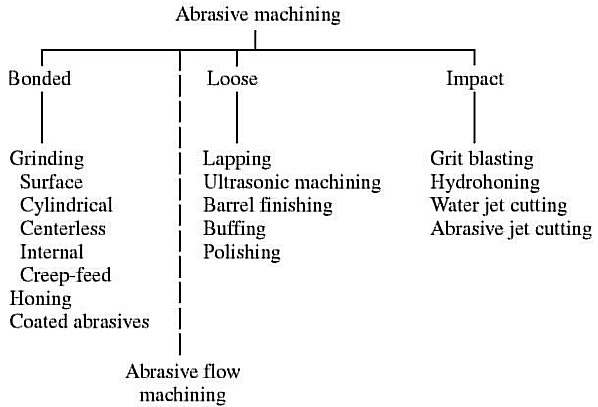
\includegraphics[width = \textwidth]{LavAbrasive}
\caption{Principali lavorazioni abrasive}
\label{fig:LavAbrasive}
\end{figure}

In generale queste lavorazioni (\ref{fig:LavAbrasive}) si cerca un'ottima finitura superficiale, a rugosità controllata combinata con una distribuzione desiderabile di tensione residue e uno strato superficiale esente da difetti.
Sono processi spesso utilizzati per la finitura dei materiali duri.

Data la tipologia dei taglienti: dispersi e con forma variabile, non c'è sicurezza che il tagliente effettivamente tagli.
C'è la possibilità che la particella tagliente tocchi il materiale ma non lo penetri, caso in figura \ref{fig:TaglTan} per cui impone solamente una deformazione elastica. 
Se invece capita che l'angolo di spoglia superiore è fortemente negativo può succedere che il tagliente sposti solamente il materiale senza effettivamente asportarlo, caso della figura \ref{fig:TaglAratro}.
Se siamo fortunati allora il tagliente riesce effettivamente a rimuovere il materiale e tagliare come in figura \ref{fig:TaglAbrasivo}.

\begin{figure}
\centering
\subfloat[][\emph{Tagliente tangente al lavorato}\label{fig:TaglTan}]
{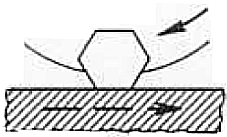
\includegraphics[width=0.3\textwidth]{TaglTan}}\:
\subfloat[][\emph{Tagliente in angolo di spoglia negativo}\label{fig:TaglAratro}]
{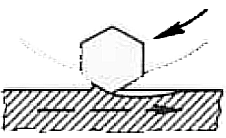
\includegraphics[width=0.3\textwidth]{TaglAratro}}\:
\subfloat[][\emph{Tagliente immerso nel materiale}\label{fig:TaglAbrasivo}]
{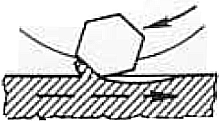
\includegraphics[width=0.3\textwidth]{TaglAbrasivo}}
\caption{Casistiche in cui si può trovare la particella tagliente}
\label{fig:PartTagl}
\end{figure}

Molto lavoro è concentrato in un piccolo spazio, quindi le temperature aumentano di molto. Si rende necessario l'utilizzo di fluidi da taglio in funzione di raffreddamento. Si possono avere pure delle scintille per via della combustione del carbonio.

\begin{figure}
\centering
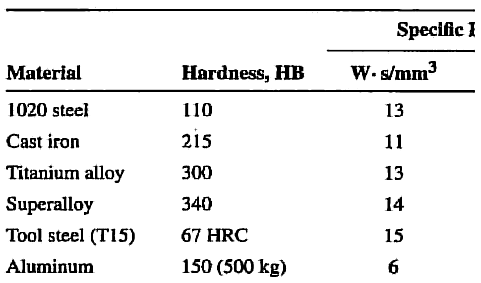
\includegraphics[width = \textwidth]{EnSpecAbrasione}
\caption{Tabella delle energie specifiche di lavorazione per diversi materiali}
\label{fig:EnSpecAbrasione}
\end{figure}

Come si vede dalla tabella \ref{fig:EnSpecAbrasione}, si nota l'inefficienza di tale lavorazione.
Come conseguenze si possono avere: ossidazioni, possibili trasformazioni di fase, formazioni di cricche, tensioni residue, ecc\dots

Le particelle devono essere particolarmente dure, soprattutto alle alte temperature.
Si richiede che tali taglienti siano fragili, in questo caso è una caratteristica apprezzata. La friabilità è necessaria per via dell'arrotondamento dei taglienti: man mano che si consumano i taglienti non tolgono più materiale. Se però questi si rompono allora vengono in superficie nuovi taglienti.
Si vuole una bassa adesione del materiale lavorato per evitare che i taglienti si attacchino al materiale lavorato. Però l'adesione all'utensile deve esser decisamente elevato.
Altre caratteristiche delle particelle è che devono essere a stabilità chimica e di forma spigolosa, proprio per garantire la minore usura e maggiore presenza di taglienti.

Alcuni materiali usati per le particelle taglienti sono: allumina in varie gradazioni di durezza. Si sfrutta allumina più tenera per lavorare materiali più duri, quella dura per materiali teneri. 
Carburo di silicio che non può essere usato per gli acciai per via della presenza del carbonio. 
Eventualmente vengono sfruttati dei materiali \textit{superabrasivi} come il CBT e C (diamanti), smepre non sugli acciai data la presenza di carbonio.

\section{Rettifica}
La categoria di lavorazioni abrasive più diffusa in industria. Si ha l'utensile che viene realizzato tramite l'adesione delle particelle taglienti a forma di una ruota che in italiano viene detta \textbf{mola}.

Sebbene lo scopo della mola sia quello di asportare del materiale, si preferisce che a perdere materiale siano entrambi gli attori, sia materiale lavorato che mola.
Da qui si può realizzare il rapporto di rettifica:
\begin{equation}
G = \frac{\overbrace{Z_w}^{\text{Materiale rimosso dalla mola}}}{\underbrace{Z_s}_{\text{materiale asportato dal pezzo}}}
\end{equation}

Le mole devono essere equilibrate per diversi motivi: le vibrazioni peggiorano le finiture superficiali, essendo in rotazione tali vibrazioni potrebbero essere amplificate ed arrivare al punto da spezzare pezzi di mola.

Nelle lavorazioni di materiali di materiali più duri si preferisce che il legante sia meno forte.

I rapporti di rettifica arrivano alla decina per acciai per utensili, sulle centinaia per acciai temprati, alle migliaia per con CBN e diamante.

Le mole hanno un certo grado di porosità, ciò permette di raccogliere le polveri generate. Eventualmente può fungere da canale per apportare fluido da rettifica.

Il legante più usato è il vetro, ciò dipende da che tipo di mola si sta utilizzando e per quale tipo di lavorazione di deve eseguire.
Altri leganti possono essere delle sostanze organiche che risultano meno forti del vetro.
Il vetro non si usa per i \textit{superabrasivi}, in quel caso viene utilizzato il bronzo sinterizzato.
Altri leganti possono essere materiali termoindurenti che però vengono spesso rinforzati da fibre di vetro, acciai ecc\dots

Per aumentare la velocità di rotazione, senza che la forza centrifuga sia eccessivamente alta, si utilizzano delle mole con parte centrale molto leggera che può essere in metallo o composito. Tenendo lo strato abrasivo superficiale di circa $3\div 5\unit{\mm}$.

La realizzazione delle mole non è così semplice, non è remota la possibilità che si stacchino dei pezzi di mola. Per cui devono sempre essere utilizzate con dei sistemi di protezione.
Esiste una normativa che definisce nel dettaglio come deve essere realizzata una mola.
Le mole vengono descritte tramite opportune scritte, normate, che ne definiscono diversi parametri che sono stati testati dal costruttore.
In figura \ref{fig:SigMola} si vedono i parametri.

\begin{figure}
\centering
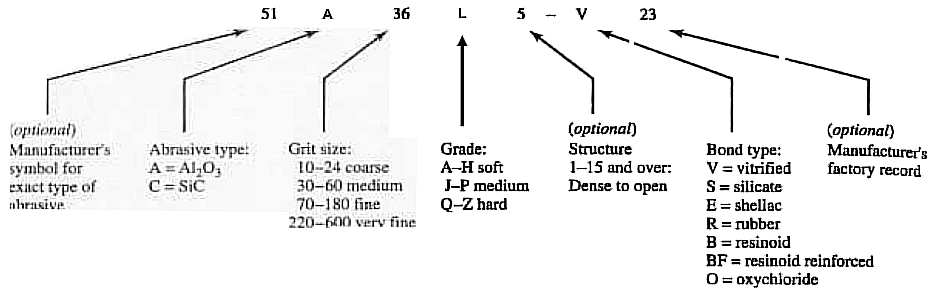
\includegraphics[width = \textwidth]{SigMola}
\caption{Descrizione della sigla per le mole}
\label{fig:SigMola}
\end{figure}

Le particelle abrasive spesso non tolgono materiale. La velocità di rimozione può essere modificata da altri aspetti tipo la forza di schiacciamento: più si preme il materiale contro la mola più materiale si asporta. Questo però modifica anche il rapporto di rettifica: in particolare lo cala drasticamente.

Sia la scelta della durezza delle particelle, che la scelta del legante deve essere calibrata in modo da favorire la generazione di nuovi taglienti.
Spesso è necessario ravvivare la mola: asportando da essa lo strato più superficiale in modo da portare alla luce nuovi taglienti più affilati.
L'operazione non è gradita: si sta lavorando non sul materiale per cui si perde tempo. In più, si abbassa lo spessore della mola.
Può essere necessaria l'operazione anche nel caso in cui il materiale lavorato diventi particolarmente pastoso alle alte temperatura, per cui il materiale aderisce alla superficie della mola e si salda sopra di essa

La ravvivatura si realizza tramite la pressione di un utensile piuttosto semplice.

\subsection{Fluidi da rettifica}
Vengono principalmente per raffreddare il lavorato per i problemi che sono stati evidenziati in precedenza, tra cui combustione, cricche a caldo ecc\dots
Si ritrova l'utilizzo della lubrificazione per avere meno carico sulla mola.
Non si ha la necessità di asportare il truciolo perché viene generata un polvere molto fine di materiale asportato che si infiltra nella porosità della mola.

Si cerca di limitare l'utilizzo di tali fluidi perché creano poltiglia tra fluido da rettifica e polvere del materiale asportato.
Grazie ai fluidi si abbassa di molto l'energia specifica per la rettifica la quale spesso viene trasformata, durante la lavorazione, in energia termica che può essere problematica visto l'ammontare di scambio termico.

Altro aspetto per cui si limita l'utilizzo dei fluidi da taglio è legato al loro smaltimento. Essendo fluidi particolari non è semplice smaltirli una volta volta consumati.

\subsection{Lavorazioni di rettifica}
\begin{figure}
\centering
\subfloat[][\emph{Rettifica orizzontale e cilindrica}\label{fig:Rettifica1}]
{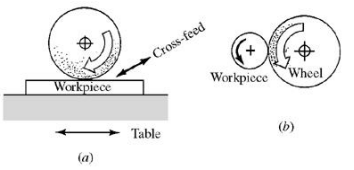
\includegraphics[width = 0.3\textwidth]{Rettifica1}}\quad
\subfloat[][\emph{Rettifica senza centri e rettifica interna}\label{fig:Rettifica2}]
{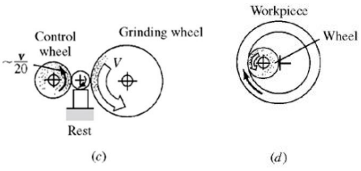
\includegraphics[width = 0.3\textwidth]{Rettifica2}}\quad
\subfloat[][\emph{Rettifica al lapitello e di forma}
\label{fig:Rettifica3}]
{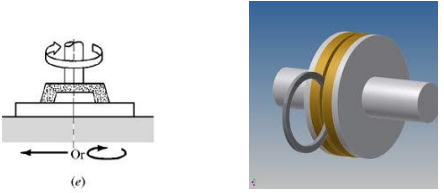
\includegraphics[width = 0.3\textwidth]{Rettifica3}}
\caption{Esempi di rettifica}
\label{fig:Rettifica}
\end{figure}

La lavorazione al lapitello, consiste in una macchina con un portapezzo magnetico in cui la mola ha una traslazione invece di una rotazione

Anche nella rettifica esistono delle mole di forma, in cui la mola ha una forma specifica in funzione della forma da ottenere.
Ovviamente il tutto dipende allo specifico prodotto da lavorare.


\subsubsection{Obbiettivi della rettifica}
\begin{description}
\item[Rettifica di precisione]: migliora le tolleranze e finitura superficiale.
\item[Rettifica di sgrossatura]: I grani usurati vengono espulsi, la velocità è più alta e l'energia specifica più bassa. Indubbiamente si sta aumentando lo spessore di truciolo indeformato.
Si usa per eliminare alimentazione e materozze dai getti e la bava dai forgiati.
\item[\eng{Creep-feed}] Con una sola passata, grande spessore di truciolo indeformato, piccolo avanzamento per giro.
Aumentando lo spessore indeformato dunque si abbassa l'energie specifica impiegata per la lavorazione.
\item[\eng{High-efficiency deep grinding}] Si usano delle mole di forma con unpo strato di CBN per asportare materiale ad alta velocità. Ci si avvicina maggiormente all'asportazione di truciolo vera e propria per via delle particelle rimosse di più grandi dimensioni.
\end{description}

Una buona finitura non garantisce qualità superficiale elevata.
La qualità della superficie aumenta con mole tenere, frequenti ravvivature e abbondante lubrificazione.

\subsubsection{Esempio}
Un esempio applicativo dei parametri utili alla realizzazione di una corretta rettifica è riportato all'appendice \ref{exe:EsempioAbrasioni} a pagina \pageref{exe:EsempioAbrasioni}.


\subsection{Nastri e carte vetrate}
particelle abrasive attaccate a carta o stoffa, sono utilizzate per operazioni di finitura a bassa velocità.
Usando colle e  supporti più forti è possibile aumentare la velocità, arrivando fino a sostituire l'asportazione di truciolo più comune.
In particolare per i nastri non è raro il fatto di trovare dei macchinari che presentano delle ruote non continue, ovvero delle ruote a settori.
Ciò fa si che il nastro non sia sempre in lavorazione, permettendo di abbassare la temperatura. Il prezzo da pagare è il maggiore tempo ciclo.

I grani vengono depositati su uno strato di adesivo applicato al supporto e vengono tenuti in posizione da uno secondo strato.
I bordi affilati dei grani e di forma allungata possono essere allineati per ottenere un angolo di spoglia leggermente negativo. Contribuendo ad aumentare l'efficienza di queste lavorazioni.

anche in questo caso si possono sfruttare i fluidi da taglio per abbassare la temperatura di lavorazione.

Un'ulteriore tipologia di utensile sono i fili. Vengono incollate sul filo le particelle taglienti che messo in movimento permette l'asportazione di materiale. Ciò taglia il materiale.

\subsection{Levigatura}
Si presenta un utensile, \ref{fig:Levigatura}, con dei settori abrasivi. I quali hanno anche un ulteriore movimento in senso radiale. L'operazione viene utilizzato per migliorare ulteriormente la finitura di fori in particolare.

L'utensile deve essere messo in pressione affinché i taglienti aderiscano alla superficie del foro da lavorare.

Il livello di finitura è superiore alle precedenti perché si tratta  di un'operazione di superabrasione. Risulta costosa e lunga. le differenze si possono vedere in figura \ref{fig:LevigatutaFine}.

\begin{figure}
\centering
\subfloat[][\emph{Esempio di utensili per levigature di cilindri interni}\label{fig:Levigatura}]
{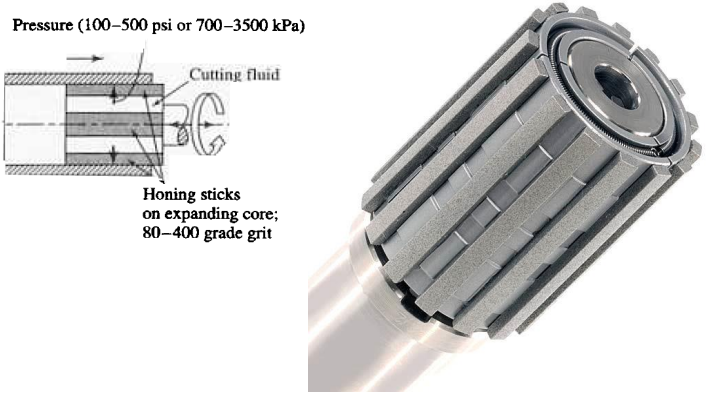
\includegraphics[width = 0.4\textwidth]{Levigatura}}\quad
\subfloat[][\emph{Finitura superficiale ottenuta con superabrasivi e abrasivi convenzionali}\label{fig:LevigatutaFine}]
{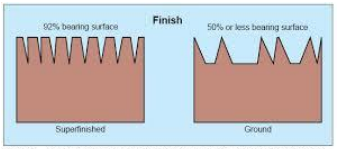
\includegraphics[width = 0.4\textwidth]{LevigaturaFine}}
\caption{Considerazioni sulla levigatura}
\label{fig:Levi}
\end{figure}


\section{Abrasione non legata}
\subsection{Lappatura}
Tramite una soluzione oleosa abrasiva posta tra il pezzo da lavorare e una superficie che è il negativo del pezzo da ottenere.
Tramite movimento planetario, rotazione del supporto più la rotazione dei singoli contenitori applicanti una certa pressione al pezzo in lavorazione, si ottiene il livello di finitura desiderato.
Alla figura \ref{fig:Lappatura} vengono mostrati lo schema di funzionamento e un macchinario per la lappatura.
Viene spesso usata per realizzare oggettistica tridimensionale come possono essere le lenti.

L'abrasione ad ultrasuoni è una lavorazione particolarmente adatta per materiali fragili.
Vedi figura \ref{fig:AbrasioneUltrasuoni}.

\subsection{Burattatura}
Si tratta di un'operazione che viene eseguita sia a secco che a liquido.
Vengono messi in un contenitore vibrante contenente: dei buratti e i pezzi da sbavare. la vibrazione mette in movimento relativo i buratti e pezzi che verranno puliti da trucioli residui e altre sbavature.
In figura \ref{fig:Burattatura}.
Si tratta di una lavorazione molto apprezzata per la capacità di pulire dei pezzi. Ciò è dato dal fatto che i buratti possono avere forme e dimensioni variegate in base alla geometria del pezzo da pulire.

\subsection{Sabbiatura}
Si tratta di un'operazione che viene spesso usata per rimuovere film superficiali o per sbavare come già visto.
Vengono scagliate delle particelle abrasive sul pezzo da ripulire

\begin{figure}
\centering
\subfloat[][\emph{Processo di lappatura}\label{fig:Lappatura}]
{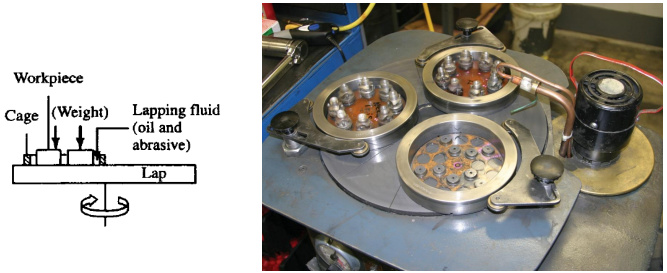
\includegraphics[width = 0.3\textwidth]{Lappatura}}\quad
\subfloat[][\emph{Abrasione ad ultrasuoni}\label{fig:AbrasioneUltrasuoni}]
{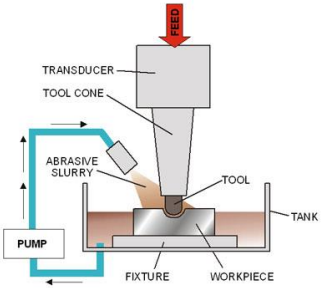
\includegraphics[width = 0.3\textwidth]{AbrasioneUltrasuoni}}\quad
\subfloat[][\emph{Esempio di burattatura}\label{fig:Burattatura}]
{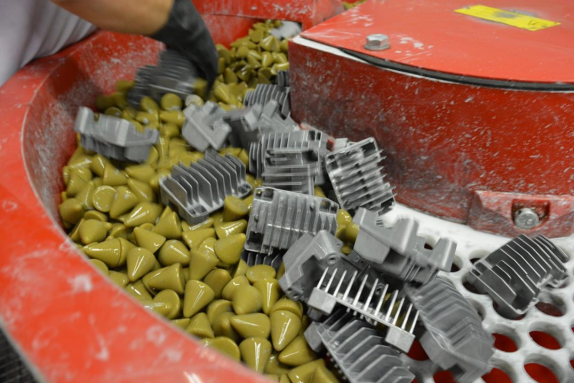
\includegraphics[width = 0.3\textwidth]{Burattatura}}
\caption{Lavorazioni abrasive non legate}
\label{fig:NonLegate}
\end{figure}


\begin{table}
\centering
\caption{Confronto delle lavorazioni abrasive a confronto con altre lavorazioni ad asportazione. 'A' indica un parametro ottimale, 'E' il peggiore}
\label{tab:ProcessiAbrasivi}
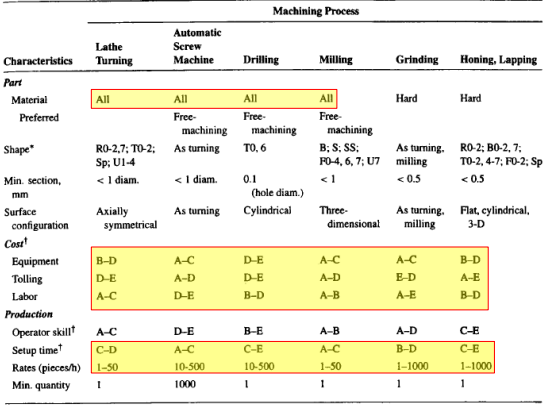
\includegraphics[width = 0.8\textwidth]{ProcessiAbrasivi}
\caption{Forme lavorabili per abrasione}
\label{fig:FormeAbrasione}
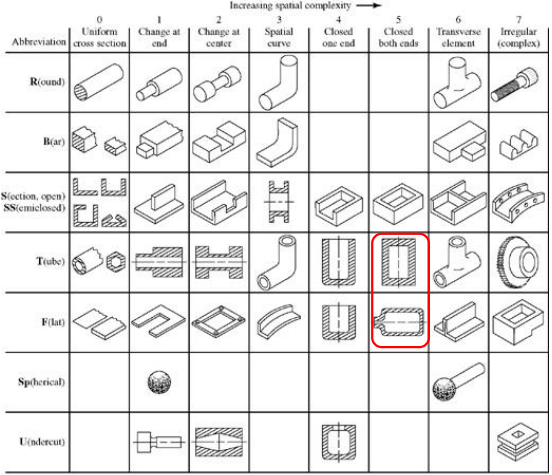
\includegraphics[width = 0.8\textwidth]{FormeAbrasione}
\end{table}


\section{Considerazioni finali}
L'asportazione di truciolo si apprezzano per tutti i materiali mentre quelle di tipo abrasivo solo per materiali duri.
Mentre l'asportazione di truciolo permette la realizzazione di praticamente tutte le forme possibili, a parte quelle in cui l'apertura di ingresso sia più piccola dell'utensile. Mentre le abrasive non vedono tutti questo campo.
In termini di dimensioni l'asportazione di truciolo non ha limiti. L'unica problematica da tenere a mente è la flessione degli utensili o dei pezzi in lavorazione.


\subsection{Aspetti progettuali}
Punti da tenere presente durante la progettazione:
\begin{itemize}
\item Scegliere un materiale ad alta lavorabilità;
\item Siccome le lavorazioni possono indurre alterazioni e produrre stati di tensione residua.
\item Bisognerebbe usare il minor numero di fissaggi possibili.
\item I raggi dovrebbero essere compatibili con l'utensile più piccolo a disposizione
\item I sottosquadri possono essere lavorati se non troppo profondi.
\item Le deflessioni degli utensili limitano il rapporto profondità/diametro.
\item Caratteristiche di forma angolate rispetto alla normale direzione di funzionamento della macchina dovrebbero essere evitate.
\item Fori ciechi su facce opposte andrebbero evitati.
\item Caratteristiche di forma angolate rispetto alla superficie deflettono l'utensile e richiedono un'operazione separata.
\item Trapanatura, fresatura ed altre operazioni producono bave.
\item La sbavatura è molto costosa e lo spessore della bava determina la modalità di rimozione.
\item La possibilità di raggiungere una determinata accuratezza dipende dalla dimensione del componente.
\item Le macchine devono essere estremamente rigide, con mandrini e guide precisi.
\item Anche gli afferraggi devono essere precisi e la forza applicata tale da non provocare distorsioni.
\item La temperatura deve essere controllata. 
\end{itemize}